% IEEE S&P 2027 submission format.
% Per the CFP: "LaTeX submissions using the IEEE templates must use
% IEEEtran.cls version 1.8b with options 'conference,compsoc'."
% Do NOT add packages/options that change margins, fonts, or line
% spacing (e.g. geometry, usenix): the CFP explicitly flags this as
% grounds for rejection without review.
\documentclass[conference,compsoc]{IEEEtran}

\usepackage{graphicx}
\usepackage{booktabs}
\usepackage{amsmath}
\usepackage{amssymb}
\usepackage{microtype}
\usepackage{xcolor}
\usepackage{caption}
\usepackage{subcaption}
\usepackage{enumitem}
\usepackage{multirow}
\usepackage{hyperref}

\usepackage{tikz}
\usetikzlibrary{arrows.meta,positioning,calc}

% Strip PDF metadata that could deanonymize the submission (author,
% affiliation leaking through document properties rather than the
% visible title page).
\hypersetup{hidelinks,pdfauthor={},pdftitle={What Does 'Delete' Mean? User Expectations and Observable Data Persistence Across Six LLM Chatbots},pdfsubject={},pdfkeywords={}}

\title{What Does `Delete' Mean? User Expectations and Observable Data Persistence Across Six LLM Chatbots}

\author{\IEEEauthorblockN{Anonymous Author(s)}
\IEEEauthorblockA{Submission \#XXX}}


\begin{document}

\maketitle

\begin{abstract}
TBWL
\end{abstract}

\section{Introduction}
\label{sec:intro}

Hundreds of millions of people now share personal, often sensitive,
information with commercial large language model (LLM) chatbots. The
right to erasure under Article 17 of the General Data Protection
Regulation (GDPR) allows individuals, under certain conditions, to
request deletion of personal data concerning them~\cite{gdpr2016}.
Commercial LLM chatbots may retain user data as conversation history,
persistent memories and conversation content used for model
training. Prior work has shown that LLMs can memorize and later
regurgitate portions of their training data~\cite{carlini2021extracting}.
Yet platforms expose multiple deletion mechanisms, including deleting a
conversation, clearing history, deleting a saved memory, or asking the
chatbot to forget information, whose actual scope is unclear.

Li et al.\ audit the privacy controls exposed by six conversational LLM
platforms and find substantial inconsistencies, including limited support
for deleting individual messages~\cite{li2026privacy}. However, their
analysis focuses on available interface controls rather than whether
invoking those controls on live accounts removes the targeted data.
Related work has documented gaps between user expectations and actual
deletion behavior in search, cloud storage, and website privacy
controls~\cite{bertram2019five,kang2015mydata,ramokapane2017stupid,habib2019empirical},
but whether similar gaps arise in commercial LLM chatbots remains largely
untested.

We therefore examine deletion from both the system and user perspectives:
whether platform controls remove the data they claim to remove, whether
observed behavior aligns with stated policy, what users believe those
controls accomplish, and where these expectations diverge from actual
platform behavior. We ask:

\begin{itemize}[leftmargin=*]
\item[] \textbf{RQ1} (system, behavior): How do commercial LLM chatbots
actually handle data deletion requests?
\item[] \textbf{RQ2} (system, policy gap): Where does observed deletion
behavior contradict each platform's stated policy?
\item[] \textbf{RQ3} (user, expectation & verification): What do users
believe deletion accomplishes, and do they verify that it worked?
\item[] \textbf{RQ4} (user, sensitivity): Does data sensitivity change
deletion method choice, willingness to delete, or expected effort/loss?
\item[] \textbf{RQ5} (divergence): Where does user expectation diverge
most from audited platform behavior, and who bears that gap?
\end{itemize}

To answer these questions, we combine a participatory survey
(RQ3--RQ4) with a technical audit of deletion controls across six
commercial LLM platforms (RQ1--RQ2, RQ5).


\section{Background and Related Work}
\label{sec:background}

\textbf{Right to erasure, at scale.} The GDPR's Article 17 right to
erasure~\cite{gdpr2016} has mostly been studied through its search-engine
delisting mechanism: Bertram et al.\ analyze five years and 3.2 million
URLs submitted to Google for right-to-be-forgotten delisting, finding
requests concentrated on a small number of sites and requesters, and
documenting the operational difficulty of adjudicating erasure at
scale~\cite{bertram2019five}. That line of work audits a single,
well-defined deletion mechanism (search delisting) end to end. Commercial
LLM chatbots instead expose several, informally specified deletion
controls over the same underlying account (conversation-level deletion,
memory-level deletion, natural-language forget requests, and
account-level deletion), which is the gap this paper's technical audit
(RQ1/RQ2/RQ5) targets.

\textbf{Auditing LLM platform controls.} Closest to this paper, Li et
al.\ walk through the stated access/edit/delete/share
controls of six conversational LLM platforms (a partially overlapping
set with the six audited here) and find them inconsistently
implemented, with most platforms not supporting deletion of an individual
message~\cite{li2026privacy}. That audit characterizes what controls each
platform's interface exposes; it stops short of testing, on live
accounts, whether invoking a given control actually removes the data it
names (the system-side gap RQ1/RQ2 target), and it does not survey users
about those controls. This paper's technical audit and participatory
survey close these two gaps respectively.

\textbf{Machine unlearning.} A deletion request that only removes a
record from a database does not, by itself, remove that record's
influence on a model already trained on it. Bourtoule et al.\ formalize
this distinction and propose \textit{SISA} training to make exact
unlearning practical, framing verifiable removal of a data point's
influence as a distinct technical problem from simply deleting the
underlying record~\cite{bourtoule2021machine}.

\textbf{User mental models of deletion.} Usable-privacy research has
repeatedly found that people's mental models of deletion do not
match how deletion is actually implemented. Kang et al.\ show that many
users hold incomplete or inaccurate models of how the internet handles
their data generally, with direct consequences for the privacy decisions
they make~\cite{kang2015mydata}. Ramokapane et al.\ study cloud-storage
deletion specifically and find users often cannot tell whether a delete
action removed data locally, from the cloud, or from other synced
devices, and adopt ad hoc coping strategies (e.g., deleting the same
item multiple times) in response to that uncertainty~\cite{ramokapane2017stupid}.
Habib et al.\ audit the deletion and opt-out controls of 150 websites
directly and find that even when a control exists, it is often
inconsistently located, under-explained, or effectively non-functional --
an interface-level failure mode distinct from, but compounding, any
backend failure to actually delete data~\cite{habib2019empirical}.

\textbf{LLM memory specifically.} On the user side specifically, Zhang
et al.\ interview 18 users of LLM chatbots with retrieval-augmented-
generation-based memory features and find diverse, often incomplete
mental models of what the memory stores and how it is used, alongside an
explicit desire for finer-grained control over reviewing, editing, and
deleting individual memories~\cite{zhang2025understanding}.

\textbf{Positioning.} Li et al.\ show that LLM platforms' stated
deletion controls are inconsistent by design~\cite{li2026privacy}; no
identified prior work tests whether those (or comparable) controls
work as stated on live accounts, or pairs such a test with a matched
participant survey of what the same controls are believed and used to
accomplish. This paper reports both halves of that pairing: a technical
audit of whether six commercial platforms' deletion controls remove the
data they claim to (RQ1, RQ2), and a participatory survey of which
deletion methods people actually choose, how those choices and their
perceived cost/protection change with data sensitivity, and where
expectation and verification behavior part ways with what the methods
are actually likely to do (RQ3, RQ4;
\S\ref{sec:sample-knowledge}), which allows the two to be compared directly
against each other (RQ5).



% \section{Diagram}
\begin{figure*}[t]
\centering
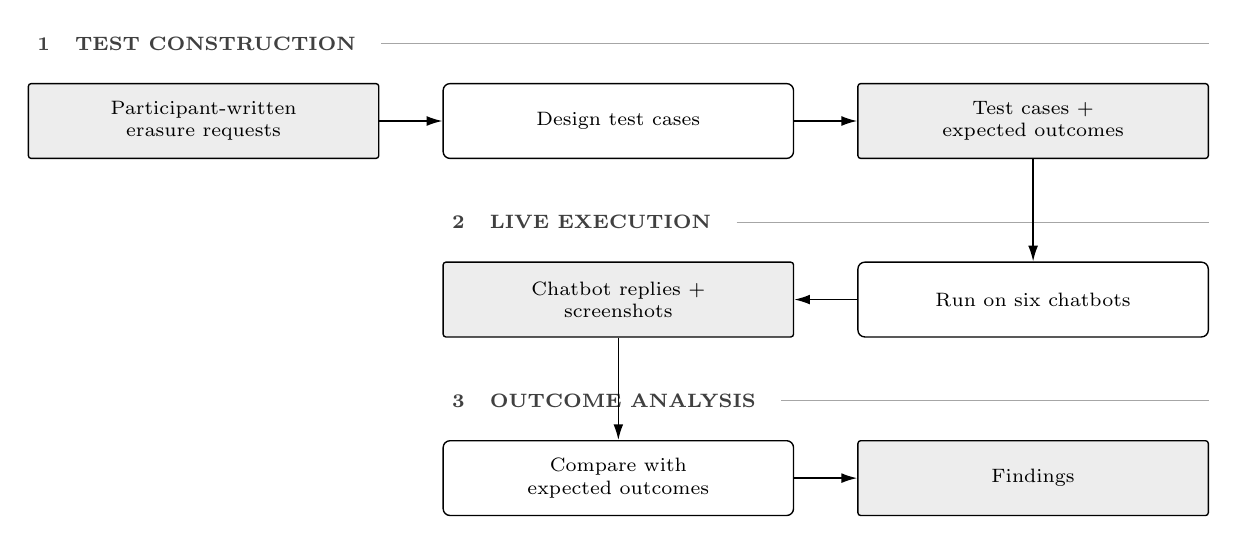
\begin{tikzpicture}[
  node distance=7mm and 8mm,
  artifact/.style={
    draw=black,
    fill=black!7,
    line width=0.5pt,
    rounded corners=1pt,
    minimum width=4.45cm,
    minimum height=0.95cm,
    align=center,
    inner sep=4.5pt,
    font=\scriptsize
  },
  action/.style={
    draw=black,
    fill=white,
    line width=0.5pt,
    rounded corners=2.5pt,
    minimum width=4.45cm,
    minimum height=0.95cm,
    align=center,
    inner sep=4.5pt,
    font=\scriptsize
  },
  flow/.style={
    -{Latex[length=2.0mm,width=1.25mm]},
    line width=0.55pt
  },
  stagelabel/.style={
    font=\scriptsize\bfseries,
    text=black!75,
    anchor=west
  }
]

% 1. Test construction
\node[artifact] (requests) {Participant-written\\erasure requests};
\node[action, right=of requests] (design) {Design test cases};
\node[artifact, right=of design] (cases) {Test cases +\\expected outcomes};

% 2. Live execution (serpentine flow)
\node[action, below=13mm of cases] (run) {Run on six chatbots};
\node[artifact, left=of run] (evidence) {Chatbot replies +\\screenshots};

% 3. Outcome analysis
\node[action, below=13mm of evidence] (compare) {Compare with\\expected outcomes};
\node[artifact, right=of compare] (findings) {Findings};

% Stage labels and rules
\node[stagelabel] (s1) at ([yshift=5mm]requests.north west) {1\quad TEST CONSTRUCTION};
\draw[black!35,line width=0.4pt] ([xshift=2mm]s1.east) -- ([yshift=5mm]cases.north east);

\node[stagelabel] (s2) at ([yshift=5mm]evidence.north west) {2\quad LIVE EXECUTION};
\draw[black!35,line width=0.4pt] ([xshift=2mm]s2.east) -- ([yshift=5mm]run.north east);

\node[stagelabel] (s3) at ([yshift=5mm]compare.north west) {3\quad OUTCOME ANALYSIS};
\draw[black!35,line width=0.4pt] ([xshift=2mm]s3.east) -- ([yshift=5mm]findings.north east);

% Main flow
\draw[flow] (requests) -- (design);
\draw[flow] (design) -- (cases);
\draw[flow] (cases) -- (run);
\draw[flow] (run) -- (evidence);
\draw[flow] (evidence) -- (compare);
\draw[flow] (compare) -- (findings);

\end{tikzpicture}
\caption{Conceptual overview of the testing pipeline.}
\label{fig:testing-pipeline}
\end{figure*}



\section{Methodology}
\label{sec:methodology}

\subsection{Participatory Survey}
\label{sec:survey-methodology}

The survey was built and administered in Qualtrics, and respondents were
recruited through Prolific (recruitment, consent and compensation are
described in the Ethics Considerations section). We set no formal sample-size
target or power calculation and aimed for roughly 200 respondents. It uses a within-subject design: the same participants rate two
scenario blocks, a less-sensitive and a more-sensitive data-deletion vignette,
presented in random order by the survey platform's block randomizer, each
repeating an identical question battery. Each scenario battery includes
three multi-item Likert scales (perceived protection with 5 items, effort
with 4 items, and benefit loss with 3 items) plus single-item measures of
deletion method choice, willingness to delete, deletion expectations, and
verification behavior. All six scale-by-scenario combinations meet
conventional reliability thresholds (Cronbach's $\alpha=0.87$--$0.92$).

\textbf{Scenarios and attention checks.} Each scenario is a short
chatbot conversation followed by the instruction to imagine deleting the
location data disclosed in it. The less-sensitive scenario (hereafter \textbf{LS}) is a weather
query: the user gives a city and asks whether to bring an umbrella. The
more-sensitive scenario (hereafter \textbf{MS}) is a health query: the user gives a home address
and asks for the nearest clinic for treatment of a sexually transmitted
infection. Results that combine both scenarios are labeled \textbf{Pooled}. Two instructed-response items check attention (``Please select
`Sometimes' for this question'' and ``Please select `Agree' for this
question''). The full scenarios and scale items are in Appendix~\ref{sec:instrument}.

\textbf{Missingness and aggregation.} Of 235 raw Qualtrics submissions,
17 incomplete/abandoned attempts are excluded first, leaving 218; 1
further response is dropped for a wrong attention-check answer, and 36 for reporting
they had never deleted chatbot data, leaving 181 eligible.
Within that eligible set, 177 respondents answered both scenarios'
method-choice items (the paired sample) and form the analysis sample; every
analysis, within a scenario or across scenarios, uses these 177 participants.
Pooled-across-scenario analyses (e.g.\ Table~\ref{tab:contingency}) treat
each participant's response in each scenario as its own observation (354
observations from the 177 paired participants) and account for the repeated
measures by clustering on participant, as described under Statistical
analysis below. Descriptive percentages are shares of the 177 participants (within a
scenario where the item was asked per scenario): demographics, usage, past use,
methods chosen, methods marked ideal and post-deletion feedback. Expectation
and verification percentages pool both scenarios and are shares of the 354
observations, as is the factor analysis. Method comparisons, including the pooled GEEs, use the 317
observations of the four methods that meet the participant threshold
below. Between-scenario comparisons
(willingness, protection, effort, benefit loss) use the Wilcoxon signed-rank
test, chosen over a paired $t$-test because Shapiro-Wilk rejected normality of
the difference scores for all three scales (40 to 51\% of participants gave the
same rating in both scenarios).

\textbf{Sample scope.} The eligibility screen keeps only respondents who
had deleted chatbot data at least once, so every survey result describes
people who found and used some deletion control. The results are silent on
the 36 of 218 complete respondents (16.5\%) who had never deleted chatbot
data, a group that may face the largest barriers to discovering deletion
controls at all.

\textbf{Statistical analysis.} Table~\ref{tab:analysis-families} lists each
inferential analysis, its test, and the family over which Holm's step-down
correction was applied. Holm-adjusted values are reported as
$p_{\mathrm{Holm}}$ and unadjusted values as $p$; a single claim never
mixes the two. We treat every survey analysis as exploratory, so $p$-values
describe the strength of evidence within a family, not a paper-wide error
rate. A nonsignificant result is read as no association detected, with
the estimate and its uncertainty where available, not as evidence of no
association: the smallest qualifying method groups contain 14 participants,
so the tests have limited power to detect small differences. Method
comparisons on ratings, expectations and verification include the four
methods chosen by at least 14 participants in a scenario (at least 29
distinct participants across both scenarios); every other method was chosen by
at most 9 in a scenario (11 distinct participants across both), so the set does
not depend on the exact cutoff. The between-scenario
tests of method choice and of ideal methods cover all listed methods. Fisher
exact tests on two-column tables (method by selected or not) are computed by
exact enumeration, so every reported $p$-value is reproducible. Survey
tests were computed with SciPy and checked against a second implementation
(101 tests, no disagreement in significance); the GEEs and
regressions with statsmodels, the CFA with semopy, and the bootstrap intervals with NumPy.

Pooled analyses (both scenarios combined) fit a generalized estimating
equation (GEE) with participant as the cluster, deletion method and scenario
as predictors, an independence working correlation, and robust (sandwich)
standard errors. The omnibus test is a Wald test that all method terms are
zero. Rating scales use an identity link and 0/1 expectation indicators a
logit link; an option that no participant chose in some method group cannot be
estimated with the logit link and enters its Holm family at $p=1$. The
independence working correlation keeps the point estimates equal to the
observed group means, which matters because method varies within a
participant (participants who switched methods appear in several groups) and
a non-independence working correlation is consistent only under stronger
assumptions about that variation. Sensitivity analyses used an exchangeable
working correlation and, for the indicators, a linear-probability model.
Post hoc contrasts compare all pairs of methods and are run only where the
Holm-adjusted omnibus test is significant.

\begin{table*}[t]
\centering
\caption{Inferential Survey Analyses, Tests, and Holm Correction Families}
\label{tab:analysis-families}
\small
\begin{tabular}{@{}p{0.29\textwidth}p{0.37\textwidth}p{0.28\textwidth}@{}}
\toprule
Analysis & Test & Holm family \\
\midrule
Scenario shift in protection, effort, benefit loss (paired, $n=177$)
  & Wilcoxon signed-rank (Shapiro-Wilk rejected normality of the difference scores)
  & 3 scales \\
Scenario shift in willingness (paired)
  & Wilcoxon signed-rank
  & Single test, unadjusted \\
Scenario shift in option selection (expectation, verification)
  & McNemar test per option
  & Options within each item (7, 8) \\
Method choice shift between scenarios
  & Stuart-Maxwell omnibus; McNemar test per method
  & 7 methods \\
Ratings by method, within a scenario
  & Kruskal-Wallis; Dunn's post hoc
  & Omnibus tests unadjusted; pairs within Dunn's test \\
Ratings by method, pooled
  & Participant-clustered GEE (Wald); pairwise contrasts
  & 3 scales; 6 method pairs \\
Expectation and verification by method, within a scenario
  & Chi-square, or $r\times c$ Fisher exact when expected counts are below 5
  & Options within each item and scenario (7, 8) \\
Expectation by method, pooled
  & Participant-clustered logit GEE (Wald)
  & 7 options \\
Ideal methods, between scenarios
  & McNemar exact test per method
  & 8 methods \\
Ratings by method, between scenarios
  & Mann-Whitney $U$ per method
  & 4 methods within each scale \\
Ratings on participant characteristics
  & Ordinary least squares, participant-clustered standard errors
  & Unadjusted \\
Correlations between scales (per scenario and pooled)
  & Spearman rank correlation
  & 9 correlations \\
Measurement model
  & Confirmatory factor analysis (ML estimation)
  & Not applicable \\
\bottomrule
\end{tabular}
\end{table*}

\subsection{Deletion-Request Prompt Corpus}
\label{sec:prompt-corpus}

One arm of the technical audit (\S\ref{sec:audit-methodology}) types real
deletion requests into each platform rather than researcher-authored
phrasings. Those requests originate in the same instrument described in
\S\ref{sec:survey-methodology}: after selecting a deletion method within
each scenario block, participants typed the exact message they would send
the assistant to carry it out and stated their rationale for that
phrasing. Respondents with a wrong attention-check answer were
excluded, as in the survey analysis. Across both scenario blocks, 209 participants submitted 415 nonblank prompts. Removing 22 exact or near-duplicate repeats within participants and 18 duplicates across participants left 375 distinct prompts. The prior-deletion-experience filter of
\S\ref{sec:sample-knowledge} is not applied to the corpus: the prompt item
asks for a hypothetical message, so it does not depend on having deleted data
before, and the corpus concerns how people phrase a request, not how they
evaluate methods they have used. A prompt is therefore included whenever its
author wrote one and was not excluded by the attention checks, whereas the survey's
181-eligible and 177-paired figures also exclude respondents who had never
deleted chatbot data or did not complete both scenarios. Each prompt was
scrubbed of residual personally identifying text (7 of 375 prompts
altered, all place names: 10 location redactions) and passed through an
automated feature-extraction step labeling candidate dimensions including
a coarse deletion-location category, used only to stratify the sampling
step below, not as the reliability-bearing codes reported next.

\textbf{Coding and reliability.} Two coders (the first author and a second
researcher) coded the prompts independently, in rounds. In the first, each
coded the same 50 prompts on all candidate dimensions without a shared
codebook; after comparing results, we kept or dropped dimensions and agreed a
shared codebook, which we applied to the same 50 prompts. Deletion location
showed the most disagreement, so we tightened its definition and recoded that
dimension alone on those prompts. We then independently coded all 138 prompts
of the audit sample (drawn as described below) on seven dimensions under the
tightened codebook: deletion location, justification, data type, grammatical
mood, tone, verb register, and accompanying secondary request.
Table~\ref{tab:ac1} reports agreement for this final round, which includes the
50 prompts used to refine the codebook.
Inter-rater reliability is reported as Gwet's $AC_1$~\cite{gwet2008ac1}
rather than Cohen's $\kappa$, because three dimensions are dominated by
one label (91--94\% of the 276 ratings), where $\kappa$ understates true
agreement~\cite{gwet2008ac1,wongpakaran2013comparison}.

\begin{table}[t]
\centering
\caption{Inter-Rater Reliability, $n=138$ per Dimension}
\label{tab:ac1}
\small
\begin{tabular}{lccc}
\toprule
Dimension & Agreement & \% & Gwet's $AC_1$ \\
\midrule
Deletion location        & 125/138 & 90.6 & 0.890 \\
Justification            & 131/138 & 94.9 & 0.943 \\
What (data type)         & 133/138 & 96.4 & 0.956 \\
Mood                     & 133/138 & 96.4 & 0.959 \\
Tone                     & 137/138 & 99.3 & 0.990 \\
Verb register            & 131/138 & 94.9 & 0.947 \\
Accompanying request     & 133/138 & 96.4 & 0.962 \\
\midrule
Pooled (966 ratings) & 923/966 & 95.5 & 0.954 \\
\bottomrule
\end{tabular}
\end{table}

\textbf{Sampling for the technical audit.} We selected 138 of the 375
prompts for the technical audit by stratified sampling on an automated
deletion-location label, with a floor so that small categories were retained.
The label definition was revised after the draw. Each selected prompt is used
as the chat-typed erasure request in the technical audit's NL-forget-prompt
cells (\S\ref{sec:audit-methodology}), verbatim except for the referent.

\subsection{Technical Audit}
\label{sec:audit-methodology}

The technical audit is a black-box behavioral test of six commercial LLM
chatbot platforms' consumer-facing deletion controls (Claude, ChatGPT,
Gemini, Copilot, Perplexity, and DeepSeek), conducted against each
platform's live web interface rather than its API, since the API does
not expose the memory, settings, and deletion surfaces the study's
research questions concern. Each platform is tested through
researcher-controlled accounts under browser automation
(Playwright)\footnote{Two of the six platforms additionally require a
stealth plugin to pass Cloudflare bot-detection checks that otherwise
block any automation-driven session; see the Ethics Considerations
section.}, driven by an orchestrator that loads each test cell's
parameters from a fixed experiment design and dispatches it to
the matching platform-specific implementation.
Figure~\ref{fig:testing-pipeline} gives a conceptual overview: participant-written
erasure requests are turned into test cases with expected outcomes, run on the
six chatbots, and the replies compared against those outcomes.

\textbf{Design.} A \textit{cell} pairs one injection method with one
erasure method on one platform. Three injection methods test distinct
memory-formation pathways: \textit{I1}, an offhand conversational mention
with no explicit request to remember it, testing whether a platform
infers memory-worthiness on its own; \textit{I2}, an explicit
``please remember'' instruction in conversation; and \textit{I3}, a
direct entry into a platform's memory/settings field where one exists. A
fourth condition, \textit{FILE}, tests document-based disclosure by
uploading a PDF containing the same disclosure content instead of typing
it. Erasure methods are drawn from each platform's own available
controls and range from conversation-level deletion, through per-item and
bulk memory deletion, to account- or privacy-dashboard-level erasure,
reflecting that no two platforms expose an identical set of deletion
surfaces. The full design comprises 85 cells: 73 platform/injection/
erasure combinations plus 12 file-upload cells, distributed unevenly
across platforms in proportion to how many memory and deletion surfaces
each one actually exposes. Three further ChatGPT cells (per-item memory
deletion crossed with I1, I2, and I3) were removed before any run, because
ChatGPT's redesigned memory interface no longer offers that action; they
are not counted.

\textbf{Policy commitments.} For RQ2, each cell in the 85-cell battery is
assigned a \textit{commitment type}, set only from what the platform's own
published documentation says about the erasure action applied to that
cell's injection surface. The source URL is recorded per cell, and the
quoted language wherever the documentation states the action's effect; a
maximal cell cites the cells it combines. The documents are listed in Appendix~\ref{sec:policy-sources}. \textsc{Deletes} means the documentation states that
the action removes the content. \textsc{Does not delete} means it states
that the action does not reach the content, as in ``deleting a
conversation does not delete saved memories''; this is a statement of
scope, not a promise that the content stays recoverable, so removal
beyond it is not a contradiction. \textsc{No commitment} means the
documentation is silent on the action for that surface, so any expectation
would be an architectural inference rather than a documented promise.
\textsc{Unrelated} means the erasure mechanism and the injection surface
are architecturally separate, so the cell tests neither.
\textsc{Not testable} means the surface cannot be reached on the test
account. Only the first two types can support a verdict on policy; cells
of the other three are reported descriptively. The verdict itself is
derived from the measured outcome by the rule in
Table~\ref{tab:consistency-rule}, not judged case by case. One documented
exception applies to requests typed into the chat to forget a fact. Where
a platform's documentation says such a request removes the saved memory but
leaves mentions of the fact in past conversations, a token recovered only
from the conversation where the fact was first disclosed is reported as
recovered but is not counted as contradicting the commitment.

\textbf{NL-forget-prompt extension.} The 138 participant-written erasure
requests sampled in \S\ref{sec:prompt-corpus} form an additional set of
cells appended to the 85-cell design: one cell per prompt per platform
(138 prompts $\times$ 6 platforms). Each prompt is typed verbatim as the
erasure request, except that its referent is replaced by the cell's disclosed referent, after a
fixed I1 (offhand conversational) disclosure. Injection type is held
constant so that erasure phrasing is the only varying factor, and recall
uses the same three-probe design (R1/R2/R3) as the 85-cell battery. All
cells on a platform share one dedicated account, distinct from the
battery's accounts, with attribution secured by each cell's unique
referent and token. This assumes that an erasure request does not erase
another cell's content, so a prompt is excluded if its wording has a high
probability of doing so. Five prompts meet this criterion: each asks for
all of the user's data, or all data in the chat, without naming a
referent. The remaining 133 each name a single referent, so their wording
does not ask for any other cell's content to be erased. They are run,
giving 798 cells (133 prompts $\times$ 6 platforms).

\textbf{Contamination control.} Accounts are reused across cells rather
than provisioned fresh per cell; attribution across cells sharing an
account is instead secured by giving every cell a unique \textit{referent}
(the conversational topic disclosed, e.g. a hobby or habit) and a unique
\textit{token} (a distinctive codename attached to that referent, 2--4
words, drawn to give each token a quantifiable, individually low guess
probability, following the canary-design rationale of prior work on
measuring unintended memorization~\cite{carlini2019secret}). A recall
probe that surfaces a cell's token is attributable to that cell alone.
Disclosure content is restricted by a narrow exclusion list (weapons,
drugs, sexual content, profanity, and a slur/explicit-term denylist)
chosen to avoid triggering platform content filters without otherwise
constraining topic naturalism.

Token uniqueness alone is not sufficient where a cell's own erasure
action is not scoped to that cell's referent at all: an account-wide
erasure, such as clearing all memories or all history, reaches every other
cell sharing that account regardless of referent. Two further account-provisioning rules
address this. First, within the 85-cell battery, any cell whose erasure
action shares an account with a sibling cell testing the same
account-wide surface, or with a cell still inside its 31-day post-erasure
recall window, is moved to its own dedicated account before either cell
runs, so that an erased or not-found recall outcome can
be attributed to the mechanism under test rather than an unrelated
blanket action that happened to share its account. Second, cross-platform
account reuse does not require this isolation: the same login credential
is deliberately reused across multiple platforms, but each platform keeps its
own account, memory and conversation history, so an action on one platform
cannot reach another. For the NL-forget-prompt extension specifically,
each platform's cells share a single dedicated account (distinct from
the 85-cell battery's accounts) rather than one account per cell, since
per-cell token uniqueness is sufficient for the 133 of 138 prompts that
each name a single referent. The remaining 5 prompts ask for all of the
user's data without naming a referent, so each has a high probability of
erasing every other prompt's still-untested content on the shared
account. They are excluded (30 of the 828 cells) rather than isolated on
dedicated accounts.

Isolating broad cells on their own accounts is necessary but not sufficient
on its own, since a request's wording can understate its actual operational
reach. Scheduling adds a second, independent layer: within any account, every
due erasure is additionally ranked by breadth. An erasure whose type matches a
fixed list of broad-action phrases ranks broadest, and the rest rank by erasure
number, from narrow (E1) to broad (E7). Cells in the same account then run
narrowest-ranked first and broadest-ranked last, so a broad action cannot
execute before a narrower sibling cell still awaiting its own turn.

\textbf{Temporal design.} Each cell runs as three separately scheduled
events rather than in immediate succession: erasure occurs 48 hours
after injection, and recall occurs 31 days after erasure. The 48-hour interval
is a fixed design choice, intended to let any asynchronous memory processing on
the platform finish before erasure. No interval could be taken from platform
documentation, which does not state one and has changed during the study:
Claude's earlier documentation described a 24-hour memory synthesis, and its
current documentation describes topic memories saved as the user chats. For
recall, three platforms (ChatGPT, Claude and
Perplexity) state that deleted data is removed from their systems within 30
days; we add one day. Gemini, Copilot and DeepSeek state no
deletion-completion time, so the same window is applied to all six for
comparability. Recall is a single visit at that point, in two parts
(\textit{new-conversation} recall for every cell, and one
\textit{same-conversation} request for typed erasures), described below.

\textbf{Recall probes.} Three probe types run at each recall point, each
in a new conversation (the new-conversation recall).
\textit{R1} (direct) always asks two open questions about the disclosed
referent, worded differently, the second a natural follow-up in the same
probe chat run regardless of what the first reply contained. R1 has no
forced-choice stage. Ranking the true value against counterfactuals, as
prior work on quantifying personal-data memorization does, relies on
model likelihoods~\cite{staufer2025wikimem}, which consumer chat
platforms do not expose. A closed question listing candidate tokens would
instead have to type the correct token into the account being tested, on
the same conversational surface I1 injection uses to plant a disclosure,
and would leave a one-in-four chance of a correct answer by guessing
alone. Recall is therefore probed by open questions only. Asking each
open probe twice, in different wordings, reflects that any single prompt gives
only a lower bound on what a model can be made to
produce~\cite{jiang2020know}, and that output can change with superficial
features of a prompt~\cite{sclar2024quantifying}.
Probing goes through each platform's consumer web interface, with the
question asked in a new conversation after the information was given
earlier, as in the evaluation of commercial chat assistants in
LongMemEval~\cite{wu2025longmemeval}.
\textit{R2} (settings) directly inspects the platform's own
memory-listing interface where one exists. \textit{R3} (indirect) always
sends two unrelated tasks that never mention the token, the second again
regardless of what the first produced, testing whether the disclosed
content leaks into unrelated generation rather than only being
recoverable when directly asked about. Running two attempts unconditionally,
for both R1 and R3, rather than only following up when the
first result is surprising, is a deliberate fix to the outcome-dependent
repetition asymmetry discussed under ``Outcome recording and repetition''
below: every cell gets the same number of checks, not just the ones whose
first answer departed from what the documentation predicted. R1 and R3
responses are matched against the token without regard to case, with
hyphens, underscores and whitespace treated as equivalent (so
``Nutcase-Taps'' matches ``Nutcase Taps'') and the token required to
appear as whole words. A reply is scored automatically only when it
contains the full token in a sentence with no negation, refusal or
question cue. A reply that contains only some of the token's words, or
contains the full token only in sentences with such a cue (for example
``I don't have any record of Nutcase Taps''), is held for human review
and coded FOUND, NOT FOUND or UNCLEAR, with UNCLEAR cases going to a
second reviewer; for R2, the reviewer records whether the fact appears
verbatim, paraphrased or not at all. The cue check only routes replies to
a person and never decides an outcome.

Within the new-conversation recall the probes run in a fixed order, R2,
then R3, then R1, the order fixed in the experiment design. The order limits
contamination between probes: R2 only reads a page and adds nothing to
the account, R3 runs before any direct question can put the token back
into the account, and R1, which names the referent outright, runs last.
This follows the finding from human memory research that taking a
retrieval test strengthens later retention of what was tested~\cite{roediger2006test},
which we treat as an analogy for a chat account's history and memory, not
as evidence about these platforms. R1 and R3 likewise mirror the
distinction between explicit and implicit tests of memory~\cite{graf1985implicit}:
R1 asks for the disclosure outright, and R3 looks for its influence on an
unrelated task. One related limitation remains and is discussed in
\S\ref{sec:limitations}: this design has no never-injected negative-control
or injected-but-not-deleted positive-control cells.

\textbf{Same-conversation recall.} When the erasure was typed into the
cell's own chat (the NL-forget prompts and the battery's typed forget
commands), that chat still exists afterwards. After the new-conversation
probes, we therefore ask one further question there: the first R1 wording,
in the conversation where the forget request was sent. It shows whether the
platform still uses the disclosure inside that chat once told to forget. It
is reported separately and is not part of the policy verdict, because the
original disclosure remains in that chat's own context, so a reply that
repeats it is expected and says nothing about what the platform keeps beyond
the chat. The request does not apply where the erasure deleted the
conversation, was a settings or interface action, or was a maximal
combination.
% TODO(authors): also report (a) a spot check of a random sample of automatically accepted
% FOUND replies, since a negation worded outside the cue list would be
% accepted, and (b) agreement between the two reviewers on a
% double-reviewed sample (Gwet's AC1).

\textbf{Measurement scope.} This design measures what a platform says and
what remains observable, not what its storage holds. Each cell yields four
measurements (``Outcome recording and repetition'' below): the
acknowledgment in the platform's reply, whether the interface visibly
changed after the erasure action, whether the content is recoverable at
the 31-day recall point, and whether the outcome is consistent with the
platform's documented commitment. Recoverability is read from three
new-conversation probes: whether the content still appears in a platform's
own memory-listing interface (R2), whether it resurfaces unprompted in
unrelated generation (R3), and whether it is recoverable when directly
asked (R1). None of these observations establishes or
rules out removal from backend storage, training datasets, or an
already-trained model's parameters: a not-found outcome shows
the token did not surface through the probes tested, not that the
underlying data was deleted from every system that might hold it, and a
found outcome shows the content remained recoverable through at
least one tested surface, not which storage location supplied it. The
canary-style token design above supports attributing a recovered token to
its originating cell~\cite{carlini2019secret}; it does not convert a
non-recovery into evidence of erasure. RQ1 and RQ2 are accordingly scoped
throughout this paper to platform-observable behavior and consistency with
documented commitments, not to backend or training-data erasure, which
this design cannot verify.

\textbf{Outcome recording and repetition.} Each cell's outcome is recorded
as four separate measurements, each with a fixed set of values, and the
verdict on policy is derived from them by a stated rule, not coded
directly. \textit{Acknowledgment} is what the platform's reply says about
the erasure request: complied, partial, refused, deflected, silently
ignored, or no reply for actions performed through the interface, which
produce none. It shows what the platform said, not that anything was
deleted. \textit{Interface change} is whether the intended surface
visibly changed after the action (changed, unchanged, or not
observable), coded from the post-erasure screenshot. A request typed into
the chat leaves nothing on the interface to inspect, so its interface change
is always not observable.
\textit{Recoverability} is the new-conversation recall outcome (``Recall
probes'' above): recovered when any probe finds the token, not recovered
when none does and the injection reached the layer the probes read, and
indeterminate otherwise, so that a missing token is never read as evidence
of deletion. The layer matters most for R2: a blank memory page counts only
when the injection could have written there (an explicit ``please remember''
or a direct memory entry, or an offhand mention that the platform showed or
claimed it saved; see ``Retention at injection'' below). A token found
anywhere counts as recovered, whatever the injection reached.
\textit{Policy consistency} combines the cell's commitment type with the
interface change and recoverability by the rules in
Table~\ref{tab:consistency-rule}. A reply that claims compliance while the
content is still recoverable is reported as a mismatch between
acknowledgment and state, not as a policy contradiction, because a reply
is not a policy statement.

\textbf{Retention at injection.} A missing token counts as evidence of
deletion only if the platform kept the fact before the erasure. Running an
extra, un-erased copy of every cell to check this would double the number
of cells, so we read it from what the platform showed when the fact was
given, in the saved transcript and the screenshot. Each cell gets one of
five values. \textit{Shown} means the interface itself displayed a memory
notice (for example ``Memory updated''). \textit{Claimed} means the reply
says, in so many words, that it saved the fact or will remember it.
\textit{Denied} means the reply says it cannot store it (``I can't save
new memories right now''). \textit{Acknowledged} means the reply only
reacted to the fact (``Noted!'') without saying it was stored. \textit{No
signal} means neither the reply nor the screen mentioned storage. Only
shown and claimed cells establish that the fact was kept. For every other
value, a token that is not recovered is reported as inconclusive, not as
evidence of deletion, and only denied points to the fact not having been
kept. Some interfaces draw the notice outside the reply text, so it is
missing from the saved transcript and is read from the screenshot instead.
A missing notice is not read as evidence that the fact was not stored, because it can appear after
the screenshot is taken. Cells that upload a file are left out, since they
are classified separately.

\begin{table}[t]
\centering
\caption{How policy consistency is derived. The commitment type fixes
which combinations of interface change and recoverability count as
consistent or contradicted. Cells of the last three types are never
contradicted, so they are reported descriptively.}
\label{tab:consistency-rule}
\small
\setlength{\tabcolsep}{3.5pt}
\begin{tabular}{@{}p{0.23\columnwidth}p{0.25\columnwidth}p{0.27\columnwidth}p{0.15\columnwidth}@{}}
\toprule
Commitment type & Contradicted & Consistent & Indeterminate \\
\midrule
\textsc{Deletes} & recovered, or interface unchanged
 & not recovered, and interface not unchanged & otherwise \\
\textsc{Does not delete} & never & recovered & not recovered \\
\textsc{No commitment}, \textsc{Unrelated}, \textsc{Not testable}
 & never & never & always \\
\bottomrule
\end{tabular}
\end{table}

Acknowledgment is recorded from the platform's single response to the
erasure request; there is no safe way to ask a platform to comply with the
same erasure request a second time without either repeating an
already-completed action or changing what is being measured. For the
chat-based erasure requests the reply text was not saved during the run,
so it was read from the post-erasure screenshot by optical character
recognition (macOS Vision, language correction disabled). A reply counts
as complete only when both its start and its end are visible on screen; a
reply that was cut off by the edge of the window, covered by an overlay, or
not yet displayed when the screenshot was taken is reported as not
captured.
% TODO(authors): if the incomplete replies are later recovered from the
% platforms' stored conversations, say so here and report the counts
% (complete / not captured) with the audit results.
Recall, by contrast, now uses a fixed
two-attempt policy applied identically to every cell regardless of
outcome (``Recall probes'' above): R1 and R3 each run twice,
unconditionally, rather than only receiving a follow-up when the first
attempt's result was surprising. This replaces an earlier design that
reran a cell's recall only when its observed outcome departed from what
the platform's documentation predicted (``Policy commitments'' above),
which held expected and unexpected recall outcomes to
different evidentiary standards; that asymmetry no longer applies to
recall, since every cell now gets the same two-attempt check independent
of what either attempt finds. Results (\S\ref{sec:audit-results}) report
both attempts for every cell, not just a single collapsed outcome. Every
phase of every cell (injection, erasure, new-conversation recall and,
where it applies, same-conversation recall) saves a transcript and a screenshot of the browser
window, retained per platform and cell for independent review. All accounts
are provisioned on each platform's free, no-cost tier; where a platform
gates a tested surface behind a paid tier, that is recorded as a result
rather than treated as a methodology gap. File-upload cells (\textit{FILE})
use a distinct, more granular verification taxonomy reflecting that a
document can be read into a conversation, into persistent memory, into
both, or into neither without a follow-up request. Extraction is
checked passively first (does the platform's own unprompted reply or
memory listing surface the token) and, only if neither does, once more
after an explicit follow-up request to summarize the document.

\textbf{Platform changes.} Copilot migrated from \texttt{copilot.microsoft.com}
to \texttt{copilot.com} during the study, so its recall runs on an interface
that differs from the one used at injection (\S\ref{sec:limitations}). Claude
replaced its memory system on 2026-09-08, which removed the memory of every
cell not yet recalled, independent of any erasure we had performed. We
re-injected the 17 Claude battery cells with fresh tokens, so their erasure
and recall timelines run from the re-injection.

\section{User Study}

\label{sec:sample-knowledge}

The analysis includes the 177 participants who completed both scenarios (\S\ref{sec:survey-methodology}; Table~\ref{tab:demographics}). Unless stated otherwise, percentages refer to participants; observation-level percentages use both scenario responses ($n=354$). The sample was relatively young, well educated, and experienced with commercial chatbots, with generally high privacy knowledge, AI literacy, and concern about sharing personal information. Participants reported sharing a broad range of information with chatbots, and prior deletion attempts covered many of the same categories.

\begin{table}[t]
\centering
\caption{Sample demographics ($n=177$).}
\label{tab:demographics}
\small
\setlength{\tabcolsep}{3.5pt}
\begin{tabular}{llcc}
\toprule
Variable & Response & $n$ & \% \\
\midrule
\multirow{6}{*}{Age}
 & 25--34 & 56 & 31.6 \\
 & 35--44 & 45 & 25.4 \\
 & 18--24 & 29 & 16.4 \\
 & 45--54 & 27 & 15.3 \\
 & 55--64 & 17 & 9.6 \\
 & 65+    & 3  & 1.7 \\
\midrule
\multirow{3}{*}{Gender}
 & Man               & 104 & 58.8 \\
 & Woman             & 72  & 40.7 \\
 & Prefer not to say & 1   & 0.6 \\
\midrule
\multirow{6}{*}{Education}
 & Bachelor's degree      & 75 & 42.4 \\
 & Graduate/professional  & 35 & 19.8 \\
 & Some college, no degree & 30 & 16.9 \\
 & Associate's/technical  & 19 & 10.7 \\
 & High school/GED        & 15 & 8.5 \\
 & Some high school or less & 3 & 1.7 \\
\midrule
Privacy Knowledge (0--6) & $M=5.06$, $Mdn=5.0$ & n/a & n/a \\
\bottomrule
\end{tabular}
\end{table}

\begin{figure}[t]
\centering
\includegraphics[width=\linewidth]{figures/fig1_ai_tenure.png}
\caption{AI chatbot usage and tenure ($n=177$).}
\label{fig:ai-tenure}
\end{figure}

\subsection{Usage of Data Deletion Methods}
\label{sec:sensitivity-effect}

\textbf{Past use.} Participants' prior deletion experience was concentrated in interface-based methods, particularly deleting individual conversations and clearing conversation history (Table~\ref{tab:method-usage}). Less common were memory-specific actions, natural-language requests to forget, and formal privacy channels. Most participants discovered deletion controls on their own, typically through platform settings, experimentation, or external documentation, while direct guidance from the platform was uncommon.


\textbf{Methods chosen in each scenario.} Deleting a single conversation was the most common choice in both scenarios, followed by clearing all conversation history (Table~\ref{tab:method-usage}). Method choice did not differ significantly between scenarios, suggesting that data sensitivity did not materially change which deletion method participants preferred.

\textbf{Ideal methods in each scenario.} Deleting a single conversation was the most commonly preferred method in both scenarios, followed by asking the chatbot to forget (Table~\ref{tab:method-usage}). Ideal-method preferences did not differ significantly across scenarios. Notably, asking the chatbot to forget ranked highly as an ideal method but was much less prominent in participants' reported past use and actual scenario choices, suggesting a gap between the deletion experience users would prefer and the methods they currently use.

\textbf{Willingness to delete.} Participants were more willing to delete their data in MS than in LS ($M=4.37$ vs.\ $3.98$; $\Delta=+0.39$, $p<.001$, $r=.55$), indicating that deletion intent increased with data sensitivity. This suggests that greater perceived privacy risk strengthens motivation to exercise deletion controls.

\begin{table*}[t]
\centering
\caption{Deletion methods: past use, method chosen in each scenario, and methods marked ideal in each scenario ($n=177$). ``Other'' was chosen by one participant in each scenario.}
\label{tab:method-usage}
\small
\begin{tabular}{lccccc}
\toprule
 & Ever used & \multicolumn{2}{c}{Chosen, $n$ (\%)} & \multicolumn{2}{c}{Ideal, \%} \\
\cmidrule(lr){3-4}\cmidrule(lr){5-6}
Method & \% & LS & MS & LS & MS \\
\midrule
Delete a single conversation & 76.8 & 84 (47.5) & 80 (45.2) & 66.1 & 60.5 \\
Clear all conversation history & 53.1 & 33 (18.6) & 40 (22.6) & 35.6 & 40.7 \\
Delete a specific saved memory & 32.2 & 19 (10.7) & 22 (12.4) & 31.1 & 41.8 \\
Ask the chatbot to forget & 31.1 & 25 (14.1) & 14 (7.9) & 46.9 & 50.3 \\
Clear all saved memories & 25.4 & 7 (4.0) & 8 (4.5) & 16.9 & 24.3 \\
Delete the account & 10.2 & 2 (1.1) & 3 (1.7) & 4.5 & 6.2 \\
Privacy dashboard & 9.6 & 6 (3.4) & 9 (5.1) & 15.3 & 17.5 \\
File a request & 2.8 & 0 (0.0) & 0 (0.0) & 2.3 & 5.1 \\
\bottomrule
\end{tabular}
\end{table*}

\subsection{Evaluation of Data Deletion Methods}

Only the four methods chosen by at least 14 participants (single conversation, clear all history, specific memory, ask to forget) enter the method comparisons below; the others are too rare to compare. Scale scores are the mean of a scale's items on a five-point agreement scale. Pooled figures use participant-scenario observations ($n=317$ across the four methods), so a participant who chose the same method in both scenarios contributes two.

\subsubsection{Measurement Model}

Because the 12 protection, effort and benefit-loss items were drawn from existing scales, we used confirmatory factor analysis (CFA) to test the intended three-factor structure. The model showed acceptable fit in the pooled data and in each scenario separately (Table~\ref{tab:cfa-fit}), with consistently strong factor loadings, convergent validity and internal consistency. The three scales were also largely distinct: protection was not significantly associated with either effort or benefit loss, while effort and benefit loss showed only a modest positive association ($\rho=.31$, $p_{\mathrm{Holm}}<.001$).

\begin{table}[t]
\centering
\caption{CFA model fit and convergent validity by scenario slice.}
\label{tab:cfa-fit}
\small
\setlength{\tabcolsep}{4pt}
\begin{tabular}{lccc}
\toprule
 & Pooled & LS & MS \\
\midrule
$n$ & 354 & 177 & 177 \\
$\chi^2$ (df${}=51$) & 225.82 & 119.32 & 155.13 \\
CFI & .941 & .954 & .931 \\
TLI & .924 & .940 & .911 \\
RMSEA & .099 & .087 & .108 \\
SRMR & .060 & .062 & .067 \\
\midrule
\multicolumn{4}{l}{\textit{AVE}} \\
\quad Protection & .643 & .633 & .652 \\
\quad Effort & .758 & .760 & .758 \\
\quad Benefit loss & .707 & .705 & .711 \\
\midrule
\multicolumn{4}{l}{\textit{Cronbach's $\alpha$}} \\
\quad Protection & .897 & .893 & .900 \\
\quad Effort & .922 & .921 & .923 \\
\quad Benefit loss & .871 & .870 & .872 \\
\bottomrule
\end{tabular}
\end{table}

\subsubsection{Perceived Privacy Protection}

Participants rated how well their chosen method protects their privacy on a five-item scale. Protection ratings were similar across methods and did not differ significantly (Table~\ref{tab:method-scales}). Ratings were modestly higher in the more-sensitive scenario, though within individual methods the difference was not significant. In a regression on both scenarios' ratings (participant-clustered standard errors), AI literacy was the only characteristic associated with protection ($b=0.28$, $p=.016$); age, education, gender and privacy concern were not. The choice of method matters less to perceived protection than whether the data feel sensitive.

\subsubsection{Benefit Loss}

Participants rated the degree to which their chosen method would reduce the chatbot's ability to provide personalised help. Benefit-loss ratings did not differ by method, scenario or any participant characteristic (Table~\ref{tab:method-scales}; regression, all $p\geq.10$). Participants anticipated a similar trade-off regardless of the method chosen or the sensitivity of the data.

\subsubsection{Effort}
\label{sec:effort}

Participants rated the time, complexity and navigational difficulty of their chosen method on a four-item scale. Effort was the only scale on which methods differed significantly (Table~\ref{tab:method-scales}). Single-conversation deletion was rated lowest and specific-memory deletion highest; in Pooled contrasts, both single-conversation and ask-to-forget were significantly less effortful than specific-memory deletion, and single-conversation was less effortful than clear-all-history. Effort did not differ between scenarios or within any individual method. Higher AI literacy was associated with lower effort ($b=-0.29$, $p=.008$); the other characteristics were not. Method choice was self-selected, so these are associations, not effects of switching methods. The pattern suggests that methods operating on finer-grained objects (a specific memory) are perceived as more effortful than those operating on coarser units (a conversation), while the natural-language option is perceived as comparably easy to the simplest interface action.

\begin{table*}[t]
\centering
\caption{Mean (SD) protection, benefit loss and effort by chosen deletion method, Pooled and by scenario. $n$ is the number of observations (Pooled; LS; MS). Method-difference rows report the Pooled GEE Wald $\chi^2$ and within-scenario Kruskal-Wallis $H$; scenario-difference rows report the Wilcoxon signed-rank test across all participants.}
\label{tab:method-scales}
\small
\setlength{\tabcolsep}{4pt}
\begin{tabular}{lcccccccccc}
\toprule
 & & \multicolumn{3}{c}{Protection} & \multicolumn{3}{c}{Benefit loss} & \multicolumn{3}{c}{Effort} \\
\cmidrule(lr){3-5}\cmidrule(lr){6-8}\cmidrule(lr){9-11}
 & $n$ & Pooled & LS & MS & Pooled & LS & MS & Pooled & LS & MS \\
\midrule
Single conversation & 164; 84; 80 & 3.63 (0.88) & 3.54 & 3.73 & 3.00 (1.03) & 2.97 & 3.02 & 1.64 (0.76) & 1.62 & 1.67 \\
Clear all history & 73; 33; 40 & 3.77 (0.87) & 3.77 & 3.77 & 3.11 (1.10) & 3.06 & 3.14 & 2.09 (0.97) & 1.98 & 2.18 \\
Specific memory & 41; 19; 22 & 3.65 (0.79) & 3.58 & 3.71 & 3.46 (0.88) & 3.54 & 3.38 & 2.49 (1.03) & 2.70 & 2.32 \\
Ask to forget & 39; 25; 14 & 3.86 (0.65) & 3.84 & 3.89 & 2.91 (0.95) & 2.91 & 2.90 & 1.74 (0.79) & 1.86 & 1.54 \\
\midrule
\multicolumn{2}{l}{Method diff.}
  & \multicolumn{3}{c}{$\chi^2\!=\!3.71$; $H\!=\!5.18$; $0.54$}
  & \multicolumn{3}{c}{$\chi^2\!=\!6.94$; $H\!=\!5.29$; $2.89$}
  & \multicolumn{3}{c}{$\chi^2\!=\!23.05$; $H\!=\!18.42$; $16.98$} \\
\multicolumn{2}{l}{}
  & \multicolumn{3}{c}{$p\!=\!.29$; $.16$; $.91$}
  & \multicolumn{3}{c}{$p\!=\!.15$; $.15$; $.41$}
  & \multicolumn{3}{c}{$p\!<\!.001$; $<\!.001$; $<\!.001$} \\
\multicolumn{2}{l}{Scenario diff.\ ($\Delta$)}
  & \multicolumn{3}{c}{$+0.13$, $p\!=\!.002$}
  & \multicolumn{3}{c}{$+0.04$, n.s.}
  & \multicolumn{3}{c}{$+0.03$, n.s.} \\
\bottomrule
\end{tabular}
\end{table*}

\subsubsection{Expectations of Data Deletion Methods}
\label{sec:expectations}

\textbf{Expected outcomes.} Expectations did not differ significantly across scenarios or deletion methods (Table~\ref{tab:contingency}), although some method-level differences were sizable and should therefore be interpreted as inconclusive rather than evidence of equivalence. Across methods, participants most often expected permanent deletion, suggesting a common expectation that deletion means the data are gone rather than merely hidden. Participants choosing specific-memory deletion were also more likely to expect the chatbot to stop referencing the data in the current conversation, consistent with a mental model linking saved memories to ongoing conversational behaviour. Training-data exclusion was a minority expectation across all methods.

\textbf{Verification.} Participants' verification strategies did not differ across scenarios but did vary by deletion method (Table~\ref{tab:contingency}). The most common response overall was not knowing how to verify that deletion had worked. Those choosing single-conversation deletion were especially likely to report no verification strategy, whereas those choosing ask-to-forget most often said they would check by asking again in the same conversation. This suggests that conversational deletion offers users an intuitive verification channel, while interface-based deletion provides less obvious feedback about whether the requested erasure has actually taken effect.

\textbf{Deleted information referenced again.} Participants were asked whether they had ever noticed a chatbot referencing information they believed they had deleted. Nearly a quarter (23.7\%) reported that they had, while 49.2\% had not and 24.3\% were unsure. That almost a quarter of experienced users report seeing deleted data resurface underscores a gap between what users expect deletion to accomplish and what the platform actually does with the data.

\textbf{Post-deletion feedback.} Two questions asked what confirmation participants currently receive and what they would want. For current feedback (select all; 18 of 177 selected more than one): 41.2\% received a clear message confirming deletion, 34.5\% a brief or vague acknowledgement, and 29.4\% no feedback at all; 4.0\% had not attempted to delete data and 2.3\% chose other. For desired feedback (again select all): participants most often wanted a popup confirmation (68.4\%) or a breakdown of what was deleted and what may be retained (41.2\%), followed by a timestamp or estimate of when deletion completes (27.7\%), an inline confirmation in the conversation (23.7\%) and an email (22.6\%); 8.5\% wanted no feedback. The demand for a detailed breakdown (41.2\%) is notable: it signals that users want transparency not just about whether data were removed, but about what may remain, a concern directly relevant to the partial-deletion outcomes the technical audit examines.

\begin{table*}[t]
\centering
\caption{Deletion method $\times$ expectation and verification (Pooled participant-scenario observations), \% of each method's observations. The ``All'' row covers all 354 observations, including methods too rare to list.}
\label{tab:contingency}
\small
\setlength{\tabcolsep}{3.5pt}
\begin{tabular}{lccccccccccc}
\toprule
 & \multicolumn{4}{c}{\textbf{Expectation}} & \multicolumn{7}{c}{\textbf{Verification}} \\
\cmidrule(lr){2-5}\cmidrule(lr){6-12}
Method (obs.) & Perm. & Not ref. & Not ref. & No longer
  & Asked, same & Asked, new & Checked & Checked & Privacy & Did not & Did not \\
 & deleted & (current) & (future) & trained
  & conv. & conv. & settings & interface & portal & know how & want to \\
\midrule
Single conv. (164)  & 58.5 & 44.5 & 54.3 & 28.0 & 12.8 & 12.8 & 10.4 & 14.6 & 2.4 & 58.5 & 12.2 \\
Clear history (73)  & 52.1 & 39.7 & 42.5 & 16.4 & 19.2 & 17.8 & 13.7 & 23.3 & 6.8 & 42.5 & 11.0 \\
Specific memory (41) & 65.9 & 68.3 & 63.4 & 19.5 & 22.0 & 34.1 & 36.6 & 12.2 & 2.4 & 29.3 & 12.2 \\
``Forget'' msg (39) & 64.1 & 53.8 & 51.3 & 35.9 & 53.8 & 33.3 & 10.3 & 10.3 & 0.0 & 23.1 & 7.7 \\
\midrule
All (354) & 59.0 & 49.2 & 54.2 & 27.7 & 20.6 & 21.8 & 17.5 & 16.1 & 5.1 & 44.6 & 10.2 \\
\bottomrule
\end{tabular}
\label{tab:verification}
\end{table*}

\section{Technical Audit Results}
\label{sec:audit-results}
% Result to report here: on Gemini, 7 of 133
% chat-based erasure requests received a prompt to connect Google Keep instead of
% a reply; nothing was deleted, and these are coded "other/asked to connect an app"
% TODO(authors): drives RQ1 (observed deletion-control behavior per
% platform/cell, recorded as the four measurements described under
% "Outcome recording and repetition" in \S\ref{sec:audit-methodology}),
% RQ2 (where observed behavior contradicts each platform's documented
% commitment; "Policy commitments" and Table~\ref{tab:consistency-rule} in
% \S\ref{sec:audit-methodology} give the exact contradiction rule; report
% the counts of each commitment type so readers can see how many cells
% could support a verdict at all, and report mismatches between
% acknowledgment and state as their own finding), and, together with
% \S\ref{sec:sample-knowledge} and \S\ref{sec:sensitivity-effect}, feeds
% RQ5 (Discussion) once real per-cell outcome data exists to report. For
% RQ5 specifically: map each survey expectation option to the specific
% platform/control/surface combination it could in principle be checked
% against (sharing six platform names across survey and audit does not by
% itself make them matched), and keep two kinds of finding visibly
% distinct rather than merging them into one "gap" number: (a) an
% observable mismatch, where the audit's documented commitment
% for a cell contradicts what participants expected, both anchored to a
% specific platform/control; and (b) an expectation this audit's
% measurement scope (\S\ref{sec:audit-methodology}'s
% "Measurement scope") cannot verify either way (chiefly training-data
% exclusion), which is a scope limitation to report, not a confirmed
% mismatch. "Who bears that gap" needs a stated subgroup (e.g., by method
% choice or by platform) or should be narrowed to whichever comparison the
% data actually support. Draft from the Acknowledgment and Interface change
% columns, the recall columns and the commitment types in MASTER, FILE
% SUBSTUDY and NL FORGET (Recoverability and Policy consistency are
% computed from them), and tester/transcripts/, once the
% audit reaches a reportable stopping point (either full completion or a
% planned interim cut), not before; do not draft this from
% partial/in-progress data presented as final.
TBWL

\section{Discussion}
\label{sec:discussion}

\textbf{Training-data exclusion is a distinct technical problem from record
deletion.} Deletion that removes a record does not, by itself, remove
that record's influence on a model already trained on it; machine-unlearning
research treats this as a distinct, harder problem than record-level
deletion~\cite{bourtoule2021machine}. In the survey, participants most
often expected permanent deletion (59.0\% of observations), while only
16--36\% of observations (depending on the method chosen) also expected
exclusion from training (\S\ref{sec:expectations}). This selection pattern does not show that
participants conflate the two outcomes. The item was select-all, so leaving an
option unselected does not mean a participant believes its opposite. The
``permanently deleted'' option was worded as deletion ``from the database and
backups,'' a claim about stored copies, so a participant may have read it as
applying to the surface they acted on and said nothing about training.
Participants may also have been unsure about training, or judged that option
redundant or unclear as worded. The training option itself did not separate
preventing future training use from removing the influence of data already
used in training, which are different expectations. We therefore report the
selection pattern without inferring a misconception; distinguishing these
readings would take explicit questions, open-ended explanations, or
interviews. Whether the expectations participants did select match what
today's chatbot deletion controls guarantee is a question the technical
audit (RQ2/RQ5) takes up directly.

\textbf{Low verification is a recurring failure mode, not a new one.}
Usable-privacy work on other deletion surfaces has repeatedly found that
a deletion control's existence does not guarantee it is understood,
locatable, or actually checked. This holds for cloud-storage
deletion~\cite{ramokapane2017stupid} and for website data-deletion and
opt-out controls audited directly~\cite{habib2019empirical}.
Participants' self-reported verification behavior fits the same pattern
in a new setting: 44.6\% of observations did not know how
to check whether a chatbot deletion worked (\S\ref{sec:expectations}). These are participants' recollections of
past behavior on the survey's verification item, not actions the study
observed directly, a distinction the technical audit's own recall probes
(\S\ref{sec:audit-methodology}) are designed to check independently. With
that caveat, the pattern suggests the verification gap is a property of
how deletion controls are generally designed and explained, not something
specific to any one platform's implementation.

\textbf{The memory-deletion effort matches a known mental-model gap.}
Interview work on LLM chatbot memory features finds that users hold
diverse, often incomplete models of what a stored memory represents
and how it was formed, and want finer-grained control over
it~\cite{zhang2025understanding}. That gives a plausible mechanism for
this paper's finding that deleting a specific saved memory was rated as
more effortful than deleting a single conversation or asking the chatbot
to forget (\S\ref{sec:effort}): if a user is unsure what a memory
entry represents or how it was derived, deciding whether and how to
delete it is harder than deleting a single conversation turn, independent
of how many clicks either action actually takes.

\textbf{Willingness to delete was higher when the data were more sensitive,
and the controls available to act on it are uneven.} Willingness to delete and
perceived protection were both higher in MS. Li et al.'s
walkthrough finds that LLM platforms' deletion controls are already
inconsistently implemented across accounts and message types~\cite{li2026privacy}.
Whether the controls users can reach keep pace with their willingness to
delete is a question this paper's user-side data cannot settle alone: it would
require separating control availability, control discoverability, and user
effort tolerance.

\textbf{Design implications.} Across the points above, the survey's selection
patterns are consistent with participants expecting deletion to reach stored
copies (most selected permanent deletion), with training exclusion being a
less frequently selected outcome, and with limited knowledge of how to verify
a deletion (44.6\% did not know how). These are implications drawn from
association patterns in self-reported data, not interventions this study
evaluated. If the patterns hold, a chatbot platform that wants its deletion
controls to function as a right-to-erasure mechanism, rather than a
lightweight convenience action, could address both by stating plainly what a
given control does and does not remove and by making the outcome possible to
confirm. Whether either change alters what users understand or do would need
to be tested directly, and the mismatch RQ5 measures would remain for
whichever of the two was left unaddressed.

\section{Limitations}
\label{sec:limitations}
\textbf{Survey.} The sample is not representative. Participants were
US-resident Prolific adults who had used at least one of the six chatbots; it
skews young (73\% under 45) and well educated (62.1\% with at least a bachelor's
degree), and participants reported high privacy knowledge (mean 5.06 of 6
correct), so the expectations and behaviors we report may not hold for chatbot
users more broadly. The survey analysis covers only respondents who had deleted
chatbot data before (36 of 218 complete respondents had not), so it says nothing
about people who never found or used a deletion control. All survey measures are
self-reported: past deletion and verification behavior are recollections and
expectations are stated beliefs, not observed actions. Method choice was
self-selected, so differences between methods are associations with the chosen
method, not effects of switching methods. The two scenarios are hypothetical
vignettes and both concern location data, a weather query and a health query
with a home address, so the differences between them may not extend to other
kinds of personal data. Finally, several comparisons had limited power: we set no
sample-size target or power calculation, the smallest method groups contained
14 participants, and a nonsignificant result is read as no association
detected, not as evidence that methods are equivalent.

\textbf{Technical audit.} The design has no never-injected negative-control or
injected-but-not-deleted positive-control cells, so a missing or recovered
token is judged against each platform's documentation and its reply at
injection, not against a control. All accounts are on each platform's free
tier, so surfaces behind a paid tier are not tested (Perplexity's Memory, and
everything that depends on it, is inaccessible on that tier), and accounts are
reused across cells, with attribution secured by a unique referent and token
and not by fresh-account isolation. Acknowledgment is read from one
observation per cell, since the same request cannot safely be sent twice, and
it shows what a platform said, not what it stored. Retention is read from the
platform's own reply and interface at injection, not from control cells;


Copilot migrated from \texttt{copilot.microsoft.com} to \texttt{copilot.com}
during the study, so its recall runs on a different interface from the one used
at injection, and Claude replaced its memory system
(\S\ref{sec:audit-methodology}); interfaces and policies can change again, and
the results describe the platforms as tested. Finally, every outcome is
platform-observable behavior: none of it can establish or rule out removal from
backend storage or training data.





\section{Conclusion}
% TODO(authors): 1-2 paragraphs restating the core contribution and
% takeaway without re-deriving statistics already given in Results.
TBWL

% ----------------------------------------------------------------
\section*{Ethics Considerations}
The survey was reviewed by the authors' institutional review board, which
determined on 2026-06-25 that it is human subjects research exempt from
regulation (exemption categories 2.i and 3A). Participants were recruited through Prolific, were
US-resident adults who had used at least one of the six chatbots, and
consented on the first page of the survey before any question; declining
ended the survey. Participation was voluntary and paid \$4 through
Prolific on completing the survey and passing the attention checks. The
survey was anonymous: no name, email address or other identifying
information was collected, responses were stored on access-restricted
university storage, and study records are kept for at least five years after
study closure. The consent form stated that de-identified data may be used
in future research or academic publications without additional consent.
Two attention and eligibility checks (failed the attention check; had never
deleted chatbot data before) were applied before the quantitative survey
analysis, excluding 37 of 218 complete responses
(\S\ref{sec:sample-knowledge}), so those analyses use only eligible,
attentive respondents' data. The deletion-request prompt corpus
(\S\ref{sec:prompt-corpus}) was extracted from the same survey; it applies the
attention check but not the experience filter, so it includes prompts from
respondents who had never deleted chatbot data. Consent was required to enter the survey, so excluded respondents gave it
under the same form as included ones. Before the prompts were used in the
audit, residual personally identifying text was redacted (\S\ref{sec:prompt-corpus}).

The technical audit (RQ1, RQ2, RQ5) interacted with six commercial LLM
chatbot platforms (Claude, ChatGPT, Gemini, Copilot, Perplexity,
DeepSeek) using researcher-controlled accounts created for this study,
not third-party or compromised accounts. Every action (sending messages,
uploading documents, invoking each platform's own memory, settings, and
deletion controls) used standard, publicly available account
functionality that an ordinary logged-in user could perform manually; no
vulnerability was exploited, no authentication or authorization boundary
was bypassed, and no other user's data was accessed at any point.
Two of the six platforms additionally required routing browser automation
through \texttt{playwright-stealth} to complete a session: without it,
generic bot-fingerprinting checks (Cloudflare) blocked the automated
browser from an already-authenticated account before it could perform
any action at all, including ones a human operator of that same account
could perform unmodified. This defeats a bot-detection heuristic aimed at
traffic patterns, not an access-control mechanism gating who may act on
the account: the stealth plugin changes how the browser presents itself,
not what credentials or authorization it holds, and every action taken
after a session loaded was identical in kind to a manual one. Potential
harm is confined to the researchers' own test-account data; the study
does not disrupt other users, access confidential information, or alter
shared infrastructure. We did not seek permission from the platforms: all
accounts were free-tier accounts, and every action was available to any
free-tier user. The IRB review covered the survey only; the audit involved
no human subjects beyond the use of the redacted survey prompts described above.
We see no path to harm for any person: the audit used only our own accounts,
accessed no other user's data, and sent ordinary requests through each
platform's public interface. Its benefit is direct evidence on whether the
deletion controls users rely on do what platforms say they do, which users
cannot currently verify for themselves.

\appendix

\section{Survey Instrument}
\label{sec:instrument}

\textbf{Scenarios.} Each scenario opened with the text ``Imagine that you
are chatting with an AI chatbot\ldots'' followed by the conversation
below and the instruction to delete the data disclosed in it.

\begin{itemize}[leftmargin=*,nosep]
\item \textit{Less sensitive (weather).} User: ``I am in Orlando now.
What's the weather today in Orlando?'' AI: ``Based on your city, it's
72\,$^{\circ}$F and sunny. There is a slight chance of rain this
evening.'' User: ``Should I bring an umbrella?'' AI: ``Probably not. The
chance of rain is only 10\%.'' \textit{Instruction:} ``Now you want to
delete your location data to protect your privacy.''
\item \textit{More sensitive (health).} User: ``I live at 7482 Orange
Blossom Lane, Orlando, FL 32801. Can you find me the nearest Medical
Center to get treatment for sexually transmitted infections?'' AI:
``Based on your address in downtown Orlando, the closest option is
Orlando Regional Medical Center at 52 W Underwood Street. If it's a
life-threatening emergency, call 911 rather than driving yourself.''
User: ``How should I prepare?'' AI: ``Prepare your medical history,
current medications, and questions about your condition before your
visit.'' \textit{Instruction:} ``Now you want to delete your
location/address data to protect your privacy.''
\end{itemize}

\textbf{Scales.} In each scenario, respondents rated the deletion method
they chose on a five-point agreement scale (Strongly Disagree,
Disagree, Neutral, Agree, Strongly Agree). The three scales, with their
items, are:

\begin{itemize}[leftmargin=*,nosep]
\item \textit{Perceived protection} (5 items): ``This data deletion method
contributes to the protection of my privacy''; ``\ldots helps me to
protect my personal information''; ``\ldots effectively reduces the risk
of my data being misused''; ``\ldots gives me complete control over my
personal data''; ``By using this data deletion method, I can decide what
personal data the AI Chatbot retains about me.''
\item \textit{Effort} (4 items): ``This data deletion method takes too
much time''; ``\ldots is overly complex to use''; ``I find it difficult to
navigate this data deletion method''; ``Understanding how this data
deletion method works requires significant effort.''
\item \textit{Benefit loss} (3 items): ``Using this data deletion method
would prevent AI Chatbots from providing responses tailored to my
activity context''; ``\ldots would reduce the relevance of assistance
tailored to my preferences''; ``Using this data deletion feature would
prevent AI Chatbots from providing the kind of help I need.''
\end{itemize}

\textbf{Attention checks.} ``Please select `Sometimes' for this question''
(frequency scale from Never to Always) and ``Please select `Agree' for
this question'' (agreement scale).





% ----------------------------------------------------------------
% TODO(authors): populate refs.bib further as the Background/Related
% Work literature review is written (a GDPR Art. 17 entry is already
% in refs.bib so \cite{gdpr2016} above resolves). IEEEtran bibliography
% style is required by the CFP template; do not substitute another.
\bibliographystyle{IEEEtran}
\bibliography{refs}


\end{document}
